\chapter{Úvod do logiky}

%Úvod do logiky, syntaxe a sémantika výrokové logiky

Slovo \emph{logika} se používá ve dvou významech:
\begin{itemize}
    \item soubor principů, které jsou základem uspořádání prvků nějakého systému (např.\ počítačového programu, elektronického zařízení, komunikačního protokolu)
    \item uvažování prováděné podle striktních pravidel zachovávajících platnost
\end{itemize}
V informatice se tyto dva významy setkávají: nejprve formálně popíšeme daný systém, a poté o něm \emph{formálně uvažujeme} (v praktických aplikacích automaticky), tj.\ odvozujeme platné \emph{inference} o systému, za použití nějakého \emph{(formálního) dokazovacího systému}.

Mezi praktické aplikace logiky v informatice patří například software verification, logic programming, SAT solving, automated reasoning, nebo knowledge-based representation. Kromě toho je logika (ve větší míře než matematika) základním nástrojem pro popis teoretické informatiky. %Více o aplikacích logiky najdete v příloze~\ref{appendix:applications}; v příloze~\ref{appendix:history} je shrnuta historie logiky.



\section{Výroková logika}

Nyní si ukážeme logiku v akci na dvou příkladech ze života (hledače pokladů, a teoretického informatika):


\subsection{Příklad: Hledání pokladu}

\begin{tcolorbox}
\begin{example}
Při hledání pokladu v dračí sluji jsme narazili na rozcestí dvou chodeb. Víme, že na konci každé chodby je buď poklad, nebo drak, ale ne obojí. Trpaslík, kterého jsme na rozcestí potkali, nám řekl, že: ``Alespoň jedna z těch dvou chodeb vede k pokladu'', a po dalším naléhání (a menším úplatku), ještě řekl, že ``První chodba vede k drakovi.'' Je známo, že trpaslíci, které člověk potká v dračí sluji, buď vždy mluví pravdu, nebo vždy lžou. Kterou cestou se máme vydat?
\end{example}
\end{tcolorbox}

\subsection{Formalizace ve výrokové logice}

Začneme tím, že situaci a naše znalosti formalizujeme ve výrokové logice. \emph{Výrok} je tvrzení, kterému můžeme přiřadit pravdivostní hodnotu: \emph{pravdivý} (\emph{True}, 1), nebo \emph{lživý} (\emph{False}, 0). Některé výroky lze vyjádřit pomocí jednodušších výroků a logických spojek, např.  ``(Trpaslík lže,) \emph{právě když} (druhá chodba vede k drakovi.)'' nebo ``(První chodba vede k pokladu) \emph{nebo} (první chodba vede k drakovi.)'' Pokud výrok takto rozložit nelze, říká se mu \emph{prvovýrok}, \emph{atomický výrok}, nebo \emph{výroková proměnná}.

Popíšeme tedy celou situaci pomocí \emph{výrokových proměnných}. Můžeme si je také představit jako jednoduché zjišťovací (ano/ne) otázky, na které musíme znát odpověď, abychom věděli vše o dané situaci. Jako naše výrokové proměnné zvolme ``Poklad je v první chodbě.'' (označme \(p_1\)), a ``Poklad je v druhé chodbě.'' (\(p_2\)). V úvahu přichází i jiné výrokové proměnné, např. ``V první chodbě je drak.'' (\(d_1\)) nebo ``Trpaslík mluví pravdu.'' (\(t\)). Ty lze ale vyjádřit pomocí \( \{p_1,p_2\} \), např.\ platí \(t\), právě když neplatí \(p_1\). Tj.\ známe-li pravdivostní hodnoty \(p_1,p_2\), pravdivostní hodnoty \(d_1,t\) jsou jednoznačně určené. A menší počet výrokových proměnných znamená menší prohledávací prostor.

Vyjádříme tedy všechny naše znalosti jako (\emph{složené}) výroky a zapíšeme je ve formálním zápisu v \emph{jazyce} výrokové logiky nad množinou prvovýroků \( \mathbb P=\{p_1,p_2\} \), za použití symbolů reprezentujících logické spojky \( \neg \) (``neplatí X'', \emph{negace}), \( \landsymb \) (``X a Y'', \emph{konjunkce}), \( \lorsymb \) (``X nebo Y'', \emph{disjunkce}), \( \limpliessymb \) (``pokud X, potom Y'', \emph{implikace}), \( \liffsymb \) (``X, právě když Y'', \emph{ekvivalence}) a závorek (,). Zde je dobré zmínit, že disjunkce není exkluzivní, tj. ``X nebo Y'' platí i pokud platí jak X tak Y, a  implikace je čistě logická: ``pokud X, potom Y'' platí kdykoliv neplatí X nebo platí Y.

Informace o tom, že v chodbě je poklad nebo drak, ale ne obojí, už je zakódovaná v naší volbě výrokových proměnných: přítomnost draka je totéž co absence pokladu. Tvrzení trpaslíka, že ``První chodba vede k drakovi.'' tedy vyjádříme jako ``Neplatí, že poklad je v první chodbě.'', formálně \(\neg p_1\). Tvrzení, že ``Alespoň jedna z těch dvou chodeb vede k pokladu.'' vyjádříme jako ``Poklad je v první chodbě nebo poklad je v druhé chodbě.'', formálně \( p_1 \lor p_2\). Informaci, že trpaslíci buď vždy mluví pravdu, nebo vždy lžou, si přeložíme tak, že buď platí oba naše výroky, nebo platí negace obou našich výroků, formálně:
\[
    (\neg p_1 \land (p_1 \lor p_2)) \lor (\neg (\neg p_1) \land \neg (p_1 \lor p_2))
\]
Označme tento výrok jako \( \varphi \) (od slova ``formule'', výrokům se někdy také říká \emph{výrokové formule}). V našem příkladě lze všechny informace vyjádřit jediným výrokem, v praxi ale často potřebujeme výroků více, někdy i nekonečně mnoho (například pokud chceme popsat výpočet nějakého programu a nevíme apriori kolik kroků bude mít), potom popíšeme situaci pomocí množiny výroků, tzv. \emph{teorie}, zde \( T=\{ \varphi \} \). Výrokům z \( T \) říkáme také \emph{axiomy} teorie~\( T \)\footnote{Terminologie v logice často pochází z jejích aplikace v matematice.}.
%\footnote{Terminologie v logice často pochází z jejích aplikace v matematice, viz příloha~\ref{appendix:history} o historii logiky.}.

\subsection{Modely a důsledky}

Jsou naše informace dostačující k určení, zda je v některé z chodeb poklad? Jinými slovy, ptáme se, zda je jeden z výroků \( p_1, p_2 \) logickým \emph{důsledkem} výroku \( \varphi \), resp.\ teorie \( T \). Co to znamená?

Představme si, že existuje více různých ``světů'' lišících se v tom, co je na konci první a na konci druhé chodby. Například, v jednom ze světů je na konci první chodby poklad a na konci druhé chodby drak. Tento svět můžeme popsat pomocí pravdivostního ohodnocení výrokových proměnných: \( p_1=1, p_2=0 \). Takovému ohodnocení říkáme \emph{model} jazyka \( \mathbb P=\{p_1,p_2\} \) a zapisujeme ho zkráceně jako \( v = (1,0) \) (\(v\) od slova ``valuation''). Celkem tedy máme čtyři různé světy, popsané \emph{modely jazyka}
\[
    \M_\mathbb P=\{(0,0),(0,1),(1,0),(1,1)\}.
\]

Je svět popsaný modelem \( v = (1,0) \) konzistentní s informacemi, které máme, tj. \emph{platí} v něm výrok \( \varphi \), resp.\ teorie \( T \)? Pravdivostní hodnotu (složeného) výroku \( \varphi \) v modelu \(v\), označme ji \( v(\varphi) \), můžeme snadno zjistit: Víme, že \( v(p_1) = 1 \) a \( v(p_2) = 0 \), takže \( v(\neg p_1) = 0 \), a také \( v(\neg p_1 \land (p_1 \lor p_2))=0 \) (jde o konjunkci dvou výroků, a první z konjunktů je v modelu \( v \) nepravdivý). Podobně \( v(p_1 \lor p_2)=1 \) (neboť \( v(p_1) = 1 \)), takže \( v(\neg(p_1 \lor p_2))=0 \), a \( v(\neg (\neg p_1) \land \neg (p_1 \lor p_2))=0 \). Výrok \( \varphi \) je disjunkcí dvou výroků, z nichž ani jeden v modelu \(v\) neplatí, tedy \( v(\varphi)=0 \).  

Bystrý čtenář jistě vidí stromovou strukturu výroku \( \varphi \) a postupné vyhodnocování \( v(\varphi) \) od listů směrem ke kořeni. Formální definice představíme v příští kapitole.

Podobně určíme pravdivostní hodnoty výroku \( \varphi \) v ostatních modelech. Zjistíme, že množina \emph{modelů výroku} \( \varphi \) (resp.\ \emph{modelů teorie} \( T \)), tj.\ množina všech modelů jazyka, ve kterých platí \( \varphi \) (resp.\ všechny výroky z teorie \( T \)), je
\[	
    \M_\mathbb P(\varphi)=\M_\mathbb P(T)=\{(0,1)\}.
\]
Vidíme, že naše informace jednoznačně určují model \( (0,1) \), tedy svět, ve kterém je v první chodbě drak a ve druhé poklad. Obecně modelů může být více, stačí nám vědět, že v každém modelu \( \varphi \), resp.{\ }\(T \), platí výrok \( p_2 \), tedy že \( p_2 \) je \emph{důsledkem} teorie \( T \); také říkáme, že \( p_2 \) \emph{platí} v teorii \( T \).

\subsection{Dokazovací systémy}

Postup, který jsme zvolili, je velmi neefektivní. Máme-li \( n \) výrokových proměnných\footnote{V praxi máme běžně tisíce proměnných.}, existuje~\( 2^n \) modelů jazyka a není prakticky možné ověřovat platnost teorie v každém z nich. Na řadu přichází tzv.\ \emph{dokazovací systémy}. V daném dokazovacím systému je \emph{důkaz} výroku~\( \psi \) z teorie \(T\) přesně, formálně definovaný syntaktický objekt, který v sobě zahrnuje snadno (mechanicky) ověřitelný ``důkaz'' (důvod), proč \( \psi \) platí v \(T\), a který můžeme hledat (pomocí počítače) čistě na základě struktury výroku \( \psi \) a axiomů teorie \(T\) (``syntaxe''), tj.\ aniž bychom se museli zabývat modely (``sémantikou'').

Po dokazovacím systému chceme dvě vlastnosti: 
\begin{itemize}
    \item \emph{korektnost}, tj.\ pokud máme důkaz \( \psi \) z \(T\), potom \( \psi \) platí v \(T\), a
    \item \emph{úplnost}, tj.\ pokud \( \psi \) platí v \(T\), potom existuje důkaz \( \psi \) z \(T\),
\end{itemize}
přičemž korektnost je nutností (bez ní nemá smysl důkazy hledat), a úplnost je dobrá vlastnost, ale efektivní dokazovací systém může být užitečný, i pokud v něm nelze dokázat vše, co platí.

Zde stručně nastíníme dva dokazovací systémy: \emph{metodu analytického tabla} a \emph{rezoluční metodu}. Později budou představeny formálně, a u obou si dokážeme i jejich korektnost a úplnost. Oba tyto dokazovací systémy jsou založeny na \emph{důkazu sporem}, tj.\ předpokládají platnost axiomů z \(T\) a negace výroku \( \psi \), a snaží se dojít ke sporu.

\subsection{Tablo metoda}

V metodě analytického tabla je důkazem \emph{tablo}: strom jehož vrcholy jsou označkované předpoklady o platnosti výroků. Podívejme se na příklad tabla na obrázku~\ref{figure:tableaux-proof-example}. 

\begin{figure}
    \centering
    \begin{forest}
    [False \( p_2 \)
        [True \( (\neg p_1 \land (p_1 \lor p_2)) \lor (\neg (\neg p_1) \land \neg (p_1 \lor p_2)) \) 
            [True \( \neg p_1 \land (p_1 \lor p_2) \)
                [True \( \neg p_1 \)
                    [True \( p_1 \lor p_2 \)
                        [False \( p_1 \)
                            [True \( p_1 \), tikz={\node[fit to=tree,label=below:\emph{fail}] {};}
                            ]
                            [True \( p_2 \), tikz={\node[fit to=tree,label=below:\emph{fail}] {};}
                            ]
                        ]
                    ]
                ]
            ]
            [True \( \neg (\neg p_1) \land \neg (p_1 \lor p_2) \)
                [True \( \neg (\neg p_1) \)
                    [True \(\neg (p_1 \lor p_2) \)
                        [False \( (\neg p_1) \)
                            [True \( p_1 \)
                                [False \(p_1 \lor p_2 \)
                                    [False \(p_1\)
                                        [False \(p_2\), tikz={\node[fit to=tree,label=below:\emph{fail}] {};}
                                        ]
                                    ]
                                ]
                            ]
                        ]
                    ]
                ]
            ]
        ]
    ]
    \end{forest}

\caption{Tablo důkaz výroku \( p_2 \) z teorie \(T\)}\label{figure:tableaux-proof-example}
\end{figure}

Začneme předpokladem, že neplatí výrok \(p_2\) (neboť dokazujeme sporem). Poté připojíme platnost všech axiomů teorie \(T\) (v našem případě je jen jeden: výrok \( \varphi \) sestrojený výše). Dále budujeme tablo tak, že zjednodušujeme výroky v předpokladech, a to podle jistých pravidel, která zaručují následující invariant: 

\begin{tcolorbox}
\emph{Každý model teorie \(T\), ve kterém neplatí \(p_2\), se musí \emph{shodovat} s některou z větví tabla (tj.\ splňovat všechny předpoklady na dané větvi).} 
\end{tcolorbox}

Výrok \( \varphi \) je disjunkcí dvou výroků, \( \varphi = \varphi_1 \lor \varphi_2 \). Pokud tedy platí v nějakém modelu, potom buď v tomto modelu platí \( \varphi_1 \), nebo v něm platí \( \varphi_2 \). Rozvětvíme strom podle těchto dvou možností. V dalším kroku máme předpoklad o pravdivosti výroku \( \neg p_1 \land (p_1 \lor p_2) \). V tom případě musí platit jak \( \neg p_1 \), tak \( p_1 \lor p_2 \), připojíme tedy na konec větve oba tyto předpoklady. Pravdivost \( \neg p_1 \) znamená lživost \( p_1 \), a tak dále.

Takto postupujeme, dokud je možné výroky v předpokladech zjednodušit, tj.\ dokud to nejsou jen výrokové proměnné. Pokud na jedné větvi najdeme dvojici opačných předpokladů o nějakém výroku \( \psi \), tj.\ že platí, a zároveň že neplatí, víme, že se s touto větví nemůže shodovat žádný model. Takové větvi říkáme \emph{sporná}.  Protože dokazujeme sporem, důkaz je takové tablo, ve kterém je každá větev sporná. Tím je zaručeno, že neexistuje model \(T\), ve kterém neplatí \(p_2\). Z toho plyne, že \(p_2\) platí v každém modelu \(T\), neboli je to důsledek \(T\), což jsme chtěli dokázat.

Zatím se spokojíme s pochopením základní myšlenky této metody, detaily představíme v budoucí kapitole.
 
\subsection{Rezoluční metoda}

Není těžké naprogramovat systematické hledání tablo důkazu. V praxi se ale používá jiný dokazovací systém, který má mnohem jednodušší a efektivnější implementaci: tzv.\ \emph{rezoluční metoda}. Tato metoda pochází z roku 1965, a je základem většiny \emph{systémů automatického dokazování}, \emph{SAT solverů}, nebo třeba interpreterů jazyka Prolog (o kterém si budeme povídat později).

Rezoluční metoda je založena na faktu, že každý výrok lze ekvivalentně vyjádřit ve speciálním tvaru, v tzv.\ \emph{konjunktivní normální formě (CNF)}. \emph{Literál} je výroková proměnná \(p\) nebo její negace \(\neg p\) (tj.\ literály jsou výroky, které jen určují hodnotu jedné výrokové proměnné). Disjunkci několika literálů, např. \( p \lor \neg q\lor \neg r\), říkáme \emph{klauzule}. A výrok je v CNF, pokud je konjunkcí klauzulí. Ke každému výroku \( \psi \) existuje \emph{ekvivalentní} výrok \( \psi' \) v {CNF}. Ekvivalentní znamená mající stejný význam (stejné modely), píšeme \( \psi \sim \psi' \). Později si ukážeme dvě metody převodu do CNF, nyní jen na našem příkladě: ve výroku
\[
    (\neg p_1 \land (p_1 \lor p_2)) \lor (\neg (\neg p_1) \land \neg (p_1 \lor p_2))
\]
nejprve nahradíme \( \neg (\neg p_1) \sim p_1 \) a \( \neg (p_1 \lor p_2) \sim (\neg p_1 \land \neg p_2) \):
\[
    (\neg p_1 \land (p_1 \lor p_2)) \lor (p_1 \land \neg p_1 \land \neg p_2)
\]
a dále opakovaně použijeme \emph{distributivitu} \( \lorsymb \) vůči \( \landsymb \) (představte si, že \( \lorsymb \) je operace násobení a \( \landsymb \) je operace sčítání):
\[
    (\neg p_1 \lor p_1) \land (\neg p_1 \lor \neg p_1) \land (\neg p_1 \lor \neg p_2) \land (p_1 \lor p_2 \lor p_1) \land (p_1 \lor p_2 \lor \neg p_1) \land (p_1 \lor p_2 \lor \neg p_2)
\]
Tento výrok už je v CNF, ale dále ho zjednodušíme: vynecháme z klauzulí duplicitní literály, a uvědomíme si, že obsahuje-li klauzule dvojici opačných literálů \( p, \neg p \), je to \emph{tautologie} (platí v každém modelu) a proto ji můžeme odstranit. Dostáváme CNF výrok
\[
    \neg p_1 \land (\neg p_1 \lor \neg p_2) \land (p_1 \lor p_2)
\]
který je ekvivalentní původnímu výroku \( \phi \)
Protože chceme dokázat \(p_2\) sporem, přidáme ještě klauzuli \(\neg p_2\):
\[
    \neg p_1 \land (\neg p_1 \lor \neg p_2) \land (p_1 \lor p_2) \land \neg p_2
\]
Výrok \(p_2\) platí v teorii \(T\), právě když je tento CNF výrok \emph{nesplnitelný} (nemá žádný model). Výroky v CNF budeme zapisovat také v \emph{množinové reprezentaci}\footnote{V praktické implementaci bychom mohli použít seznam klauzulí, kde každá klauzule je seznam (unikátních) literálů v nějakém zvoleném uspořádání. Představte si opět tisíce výrokových proměnných a klauzulí.}:
\[
    \left \{ \{\neg p_1\},\{\neg p_1,\neg p_2\},\{p_1, p_2\},\{\neg p_2\} \right \}
\]
\emph{Rezoluční pravidlo} říká, že pokud máme dvojici klauzulí, z nichž jedna obsahuje literál \(p\) a druhá opačný literál \(\neg p\), potom z nich logicky plyne také jejich\ \emph{rezolventa}: klauzule vzniklá odstraněním literálu \(p\) z první a \(\neg p\) z druhé klauzule a sjednocením zbylých literálů. Například, z \( p \lor \neg q\lor \neg r\) a \( \neg p \lor \neg q \lor s\) můžeme odvodit rezolventu \( \neg q \lor \neg r \lor s\). \emph{Rezoluční zamítnutí} formule v CNF je potom posloupnost klauzulí, která končí \emph{prázdnou klauzulí \( \square \)} (znamenající spor) a kde každá klauzule je buď z dané formule, nebo je rezolventou nějakých dvou předchozích klauzulí. V našem případě:
\[
    \{\neg p_1\},\{p_1, p_2\},\{p_2\},\{\neg p_2\},\square
\]
Třetí klauzule je rezolventou první a druhé, pátá je rezolventou třetí a čtvrté. Rezoluci lze také přirozeně znázornit pomocí \emph{rezolučního stromu}, kde listy jsou klauzule z dané formule, a vnitřní vrcholy jsou rezolventy svých potomků:

\begin{center}
\begin{forest}
for tree={grow=north}
[\( \square \)
    [\( \{\neg p_2\} \)]
    [\( \{p_2\} \)
    [{\( \{p_1, p_2\} \)}]
    [\( \{\neg p_1\} \)]
    ]
]
\end{forest}
\end{center}

Pokud by formule měla model, musely by v něm platit její klauzule, tedy i postupně všechny rezolventy v posloupnosti, a nakonec prázdná klauzule. Ta ale neplatí v žádném modelu. Máme tedy důkaz sporem a víme, že ve druhé chodbě najdeme poklad.


\subsection{Příklad: Barvení grafů}\label{subsection:example-graph-coloring}

Ve druhém příkladu se trochu přiblížíme aplikacím. Na rozdíl od logických hádanek ve formě slovních úloh, různé varianty problému barvení grafů se objevují v rozmanitých úlohách z praxe, od rozvrhovacích problémů přes návrh fyzických a síťových systémů po zpracování obrazu.

\begin{tcolorbox}
\begin{example}\label{example:graph-coloring-intro}
Najděte vrcholové obarvení následujícího grafu třemi barvami, tj.\ přiřaďte vrcholům barvy R, G, B tak, aby žádná hrana nebyla monochromatická.
\begin{center}
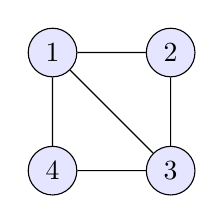
\begin{tikzpicture}[every node/.style={circle,fill=blue!10,draw,minimum size=0.5cm,node distance=1.5cm}]
\node (1) {$1$};
\node[right of=1] (2) {$2$};
\node[below of=2] (3) {$3$};
\node[left of=3] (4) {$4$};
\path[draw] (1) -- (2) -- (3) -- (4) -- (1) -- (3);
\end{tikzpicture}
\end{center}
\end{example}
\end{tcolorbox}

Graf si reprezentujeme jako množinu vrcholů a množinu hran, kde každá hrana je dvojice vrcholů. Lépe se nám bude pracovat s uspořádanými dvojicemi, zvolíme tedy (libovolnou) orientaci hran.
\[
\structure G = \langle V; E \rangle = \langle \{1,2,3,4\}; \{(1,2),(1,3),(1,4),(2,3),(3,4)\} \rangle
\]



Začneme opět formalizací ve výrokové logice. Označme si množinu barev jako \( C=\{R,G,B\} \).  Přirozená volba výrokových proměnných je ``vrchol \(v\) má barvu \(c\)'', označme \(p_v^c\), pro každý vrchol \(v \in V\) a každou barvu \(c\in C\). Naše (uspořádaná) množina výrokových proměnných má 12 prvků:
\[
\mathbb P=\{p_v^c\mid c\in C,v\in V\}=\{p_1^R,p_1^G,p_1^B,p_2^R,p_2^G,p_2^B,p_3^R,p_3^G,p_3^B,p_4^R,p_4^G,p_4^B\}
\]
Máme celkem \( |\M_\mathbb P|=2^{12}=4096 \) modelů jazyka (reprezentovaných 12-dimenzionálními 0--1 vektory). Většinu z nich nelze interpretovat jako obarvení grafu. Například \( v=(1,1,0,0,\dots,0) \) říká, že vrchol 1 je obarvený červeně, a také zeleně. Začneme tedy teorií vyjadřující, že každý vrchol má nejvýše jednu barvu. Existuje více způsobů, jak to můžeme vyjádřit. My řekneme pro každý vrchol, že nesmí mít (alespoň) jednu z každé dvojice barev. Tím dostaneme teorii v {CNF}:

\begin{align*}
T_1 = \{ 
&(\neg p_1^R \lor \neg p_1^G) \land (\neg p_1^R \lor \neg p_1^B) \land (\neg p_1^G \lor \neg p_1^B),\\
&(\neg p_2^R \lor \neg p_2^G) \land (\neg p_2^R \lor \neg p_2^B) \land (\neg p_2^G \lor \neg p_2^B),\\
&(\neg p_3^R \lor \neg p_3^G) \land (\neg p_3^R \lor \neg p_3^B) \land (\neg p_3^G \lor \neg p_3^B),\\
&(\neg p_4^R \lor \neg p_4^G) \land (\neg p_4^R \lor \neg p_4^B) \land (\neg p_4^G \lor \neg p_4^B)\} \\
    = \{ &(\neg p_v^R \lor \neg p_v^G) \land (\neg p_v^R \lor \neg p_v^B) \land (\neg p_v^G \lor \neg p_v^B) \mid v \in V \} 
\end{align*}
Teorii \(T_1\) bychom mohli říkat teorie částečných vrcholových obarvení grafu \(\structure G\). Teorie \(T_1\) má \(|\M_\mathbb P(T_1)|= 4^4=2^8=256\) modelů. (Proč?) Pokud chceme úplná obarvení, přidáme podmínku, že každý vrchol má alespoň jednu barvu.\footnote{Symbol \(\bigvee \) používáme podobně jako symboly \(\sum \) pro součet a \(\prod \) pro součin: ke zjednodušení zápisu výroku, který je ve formě disjunkce. Např.\ pokud \(v=1\), potom \( \bigvee_{c\in C} p_v^c \) reprezentuje výrok \( p_1^R \lor p_1^G \lor p_1^B \). Analogicky \(\bigwedge \) pro konjunkci.}

\begin{align*}
T_2 &= T_1\cup \{p_1^R \lor p_1^G \lor p_1^B, p_2^R \lor p_2^G \lor p_2^B, p_3^R \lor p_3^G \lor p_3^B, p_4^R \lor p_4^G \lor p_4^B\} \\
    &= T_1\cup \{ p_v^R \lor p_v^G \lor p_v^B \mid v \in V \} \\
    &= T_1\cup \{\bigvee_{c\in C} p_v^c \mid v \in V \}  
\end{align*}

Teorie \( T_2 \) má \(3^4=81\) modelů. Jde o \emph{extenzi} teorie \( T_1 \), neboť každý důsledek teorie \( T_1 \) platí i v teorii \( T_2 \). Platí dokonce, že \( \M_\mathbb P(T_2)\subseteq\M_\mathbb P(T_1) \).\footnote{Zde vidíme typickou ukázku antimonotónního vztahu tzv.\ Galoisovy korespondence: čím více vlastností (výroků) požadujeme, tím méně objektů (modelů) splňuje tyto vlastnosti.} Zbývá přidat podmínku zakazující monochromatické hrany. Pro každou hranu a každou barvu specifikujeme, že alespoň jeden z vrcholů hrany nesmí mít danou barvu. Zde pro názornost naposledy napíšeme úplný seznam výroků, nadále budeme využívat zkráceného zápisu.
\begin{align*}
    T_3 = T_2\cup \{ & (\neg p_1^R \lor \neg p_2^R) \land (\neg p_1^G \lor \neg p_2^G) \land (\neg p_1^B \lor \neg p_2^B),\\
    & (\neg p_1^R \lor \neg p_3^R) \land (\neg p_1^G \lor \neg p_3^G) \land (\neg p_1^B \lor \neg p_3^B),\\
    & (\neg p_1^R \lor \neg p_4^R) \land (\neg p_1^G \lor \neg p_4^G) \land (\neg p_1^B \lor \neg p_4^B),\\
    & (\neg p_2^R \lor \neg p_3^R) \land (\neg p_2^G \lor \neg p_3^G) \land (\neg p_2^B \lor \neg p_3^B),\\
    & (\neg p_3^R \lor \neg p_4^R) \land (\neg p_3^G \lor \neg p_4^G) \land (\neg p_3^B \lor \neg p_4^B)\} \\  
= T_2\cup \{ &\bigwedge_{c\in C} 
(\neg p_u^c \lor \neg p_v^c) \mid (u,v) \in E \}
\end{align*}
Výsledná teorie \( T_3 \) je \emph{splnitelná} (má model), právě když graf \( \structure{G} \) je 3-obarvitelný. Má 6 modelů jednoznačně odpovídajících 3-obarvení grafu \( \structure G \). Model \( v = (1,0,0,0,1,0,0,0,1,0,1,0) \) odpovídá následujícímu obarvení, ostatní obarvení získáme permutací barev.
\begin{center}
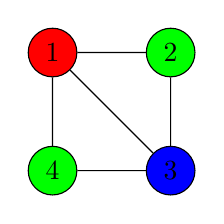
\begin{tikzpicture}[every node/.style={circle,fill=blue!10,draw,minimum size=0.5cm,node distance=1.5cm}]
\node[fill=red] (1) {$1$};
\node[fill=green,right of=1] (2) {$2$};
\node[fill=blue,below of=2] (3) {$3$};
\node[fill=green,left of=3] (4) {$4$};
\path[draw] (1) -- (2) -- (3) -- (4) -- (1) -- (3);
\end{tikzpicture}
\end{center}

Jakmile máme teorii \(T_3\) formalizující 3-obarvení grafu \( \structure{G} \), můžeme snadno řešit související otázky, například najít všechna obarvení, ve kterých je vrchol 1 modrý a vrchol 2 zelený: odpovídají modelům teorie \( T_3 \cup \{ p_1^B, p_2^G\} \). Nebo můžeme dokázat, že vrcholy 2 a 4 musejí být obarveny stejnou barvou. Můžeme použít tablo metodu: v kořeni tabla bude předpoklad
\[
\text{False  }(p_2^R \land p_4^R)\lor(p_2^G \land p_4^G)\lor(p_2^B \land p_4^B)
\]
Nebo můžeme najít rezoluční zamítnutí teorie vzniklé převedením axiomů teorie \( T_3 \) do CNF, a přidáním CNF ekvivalentu \emph{negace} výroku \( (p_2^R \land p_4^R)\lor(p_2^G \land p_4^G)\lor(p_2^B \land p_4^B) \)	(neboť jde o důkaz sporem, tedy pro spor předpokládáme, že \emph{nemají} stejnou barvu).



\section{Predikátová logika}

Nyní si velmi stručně a neformálně představíme \emph{predikátovou logiku}. Predikátová logika se zabývá vlastnostmi objektů a vztahy mezi objekty. Například:
\begin{quote}\it
    Všichni lidé jsou smrtelní.\\
    Sókratés je člověk.\\
    Sókratés je smrtelný.
\end{quote}
Ve skutečnosti výroková logika vznikla později (asi o století) než Aristotelova predikátová logika, a byla poté na dlouho převážně zapomenuta.


\subsection{Nevýhody formalizace ve výrokové logice}\label{subsection:disadvantages-of-propositional-logic}

Nevýhodou formalizace našeho problému ve výrokové logice je fakt, že výsledná teorie \( T_3 \) je poměrně velká, a navíc byla vytvořena ad hoc pro graf  \( \structure{G} \). Představme si, že potřebujeme graf \( \structure{G} \) změnit, například přidáním vrcholu 5 spojeného hranami s vrcholy 2 a 3:

\begin{center}
    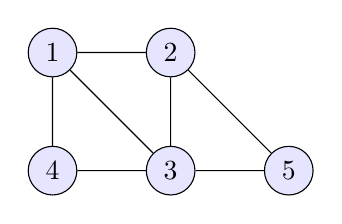
\begin{tikzpicture}[every node/.style={circle,fill=blue!10,draw,minimum size=0.5cm,node distance=1.5cm}]
    \node (1) {$1$};
    \node[right of=1] (2) {$2$};
    \node[below of=2] (3) {$3$};
    \node[left of=3] (4) {$4$};
    \path[draw] (1) -- (2) -- (3) -- (4) -- (1) -- (3);
    \node[right of=3] (5) {$5$};
    \path[draw] (2) -- (5) -- (3);
    \end{tikzpicture}
\end{center}

Abychom byli schopni formalizovat nový problém, musíme přidat do našeho jazyka tři nové výrokové proměnné: \(\mathbb P'=\mathbb P \cup \{ p_5^R,p_5^G,p_5^B\} \), a vytvořit nové teorie \( T'_1, T'_2, T'_3 \) přidáním axiomů týkajících se vrcholu 5 a hran \( (2, 5), (3,5) \). Problémem je, že strukturu grafu \( \structure{G} \) a přirozené vlastnosti jako ``z vrcholu \(u\) vede hrana do vrcholu \(v\)'', nebo ``vrchol \(u\) je zelený'' jsme (`natvrdo', `nepřirozeně') zakódovali do 0--1 proměnných. Tento nedostatek odstraňuje \emph{predikátová logika}.

\subsection{Stručné představení predikátové logiky}

\emph{Modelem} v predikátové logice není 0--1 vektor, ale \emph{struktura}. Příkladem struktur jsou naše (orientované) grafy:
\begin{align*}
    &\structure G = \langle V^\structure G; E^\structure G \rangle = \langle \{1,2,3,4\}; \{(1,2),(1,3),(1,4),(2,3),(3,4)\} \rangle \\ 
    &\structure{G}' = \langle V^{\structure{G}'}; E^{\structure{G}'} \rangle = \langle \{1,2,3,4,5\}; \{(1,2),(1,3),(1,4),(2,3),(3,4),(2,5),(3,5)\} \rangle
\end{align*}
Oba grafy sestávají z množiny vrcholů, a z binární relace na této množině. Jde o struktury v \emph{jazyce teorie grafů} \( \mathcal L=\langle E \rangle \), kde \(E\) je binární \emph{relační symbol}. \emph{Jazyk} predikátové logiky specifikuje jaké relace (kolik a jakých arit --- unární, binární, ternární, atd.) mají struktury mít, a jaké symboly pro ně budeme používat. Kromě toho používáme symbol rovnosti \(=\) a struktury mohou obsahovat také funkce a konstanty (jako například funkce \( +,-,\cdot \) a konstanty $0,1$ v \emph{tělese} reálných čísel), ty si ale necháme na později.

Predikátová logika používá tytéž logické spojky jako výroková logika, ale základním stavebním kamenem \emph{predikátových formulí} nejsou výrokové proměnné, nýbrž tzv.\ \emph{atomické formule}, například: \( E(x,y) \) představuje tvrzení, že v grafu vede hrana z vrcholu \(x\) do vrcholu \(y\). Zde \(x,y\) jsou \emph{proměnné} reprezentující vrcholy daného grafu. Kromě toho ve formulích můžeme používat \emph{kvantifikátory}: \( (\forall x) \) ``pro všechny vrcholy \(x\)'' a \( (\exists y) \) ``existuje vrchol \(y\)''.\footnote{Kvantifikátory si můžeme představit jako ``konjunkci'' resp.\ ``disjunkci'' přes všechny vrcholy grafu.} 

Nyní můžeme formalizovat tvrzení, která dávají smysl pro libovolný graf. Například: 
\begin{itemize}
    \item ``V grafu nejsou smyčky'': \[ (\forall x)(\neg E(x,x)) \] 
    \item ``Existuje vrchol výstupního stupně 1'': \[ (\exists x)(\exists y)(E(x,y) \land (\forall z)(E(x,z) \limplies y=z)) \] 
\end{itemize}
V daném grafu \(\structure{G}\) a při dosazení vrcholu \(u\) za proměnnou \(x\) a vrcholu \(v\) za proměnnou \(y\) vyhodnotíme \( E(x,y) \) jako True, právě když \( (u,v)\in E^{\structure{G}} \).


\subsection{Formalizace barvení grafů v predikátové logice}


Vraťme se zpět k barvení grafů. Přirozený způsob jak formalizovat náš problém 3-obarvitelnosti je v jazyce \( \mathcal L' =\langle E, R, G, B \rangle \), kde \(E\) je binární a \(R,G,B\) jsou unární relační symboly, tedy \(R(x)\) znamená ``vrchol \(x\) je červený''. Strukturou pro tento jazyk je (orientovaný) graf spolu s trojicí množin vrcholů, např.
\begin{align*}
\structure G_C &= \langle V^{\structure G_C}; E^{\structure G_C}, R^{\structure G_C}, G^{\structure G_C}, B^{\structure G_C} \rangle \\
&= \langle \{1,2,3,4\}; \{(1,2),(1,3),(1,4),(2,3),(3,4)\}, \{1\}, \{2,4\}, \{3\} \rangle    
\end{align*}
reprezentuje graf \( \structure{G} \) s validním obarvením z obrázku výše. Budeme říkat, že \( \structure{G}_C \) je \emph{expanze} \(\mathcal L\)-struktury \( \structure{G} \) do jazyka \( \mathcal L' \).

Podobně jako ve výrokové logice musíme nejprve zajistit, aby naše modely reprezentovaly obarvené grafy. Začneme požadavkem, aby každý vrchol byl obarven nejvýše jednou barvou:
\[
(\forall x)((\neg R(x) \lor \neg G(x)) \land (\neg R(x) \lor \neg B(x)) \land (\neg G(x) \lor \neg B(x)))
\]
Obarvení alespoň jednou barvou vyjádříme takto:
\[
(\forall x)(R(x) \lor G(x) \lor B(x))
\]
A hranovou podmínku formalizujeme pomocí predikátu \( E(x,y) \) například takto:
\[	
(\forall x)(\forall y)(E(x,y) \limplies ((\neg R(x) \lor \neg R(y)) \land (\neg G(x) \lor \neg G(y)) \land (\neg B(x) \lor \neg B(y))))
\]
Modely takto vzniklé teorie reprezentují orientované grafy s vrcholovým 3-obarvením. 


\section{Další druhy logických systémů}

Predikátové logice, kde proměnné reprezentují jednotlivé vrcholy, říkáme logika \emph{prvního řádu} (anglicky  \emph{first-order (FO) logic}). V logice \emph{druhého řádu} (anglicky \emph{second-order (SO) logic}) máme také proměnné reprezentující množiny vrcholů nebo i množiny \(n\)-tic vrcholů (tj.\ relace, funkce). Například tvrzení, že daný graf je bipartitní, můžeme formalizovat v logice druhého řádu následující formulí, ve které $S$ je \emph{proměnná druhého řádu} reprezentující množinu vrcholů a $S(x)$ vyjadřuje, že ``vrchol $x$ je prvkem množiny $S$'':
$$
(\exists S)(\forall x)(\forall y)(E(x,y)\limplies (S(x)\liff\neg S(y)))
$$
Jako jiný, důležitý příklad uveďme tvrzení, že každá neprázdná zdola omezená podmnožina má infimum,\footnote{Což platí v uspořádané množině reálných čísel, ale neplatí v racionálních číslech, např.\ \( \{x \mid x^2 > 2, x > 0\} \).} které můžeme formalizovat v logice druhého řádu takto:\footnote{I když je tato formule velmi složitá, pokuste se porozumět jednotlivým částem.}
\begin{align*}
&(\forall S)((\exists x)S(x) \land (\exists x)(\forall y)(S(y) \limplies x\leq y) \limplies  {}\\ 
&(\exists x)((\forall y)(S(y) \limplies x\leq y) \land (\forall z)((\forall y)(S(y) \limplies z\leq y)\limplies z\leq x)))
\end{align*}
A v logice \emph{třetího řádu} máme i proměnné reprezentující množiny množin (což je užitečné např.\ v topologii), atd.

Kromě výrokové a predikátové logiky existují i další typy logických systémů, například intuicionistická logika (která povoluje jen konstruktivní důkazy), temporální logiky (kde mluvíme o platnosti `vždy', `někdy v budoucnosti', `dokud' apod.), modální logiky (`je možné', `je nutné'), nebo fuzzy logiky (kde máme výroky `0.35 pravdivé'). Tyto logiky mají důležité aplikace v informatice, např.\ v umělé inteligenci (modální logiky pro uvažování autonomních agentů o svém okolí), v paralelním programování (temporální logiky), nebo v automatických pračkách (fuzzy logiky). %Více viz Příloha~\ref{appendix:other-logics}. 
V tomto kurzu se omezíme na výrokovou logiku a predikátovou logiku prvního řádu.


\section{O přednášce}

Přednášku lze rozdělit do třech částí. 

První část se zabývá výrokovou logikou. Nejprve představíme syntaxi a sémantiku, dále problém splnitelnosti CNF formulí (známý NP-úplný problém SAT) a jeho polynomiálně řešitelné fragmenty (2-SAT, Horn-SAT). Budeme pokračovat tablo metodu, u níž si dokážeme korektnost a úplnost, a také několik aplikací, například Větu u kompaktnosti. A na závěr představíme rezoluční metodu ve výrokové logice.

Ve druhé části představíme predikátovou logiku. Začneme opět syntaxí a sémantikou, ukážeme si jak lze adaptovat tablo metodu pro predikátovou logiku, a skončíme znovu rezoluční metodou. Kromě toho zmíníme několik praktických aplikací: databázové dotazy, logické programování (jazyk Prolog), a softwarovou verifikaci.

Třetí část je úvodem do teorie modelů, definovatelnosti, axiomatizovatelnosti, a algoritmické rozhodnutelnosti. Na závěr si představíme slavné Gödelovy věty o neúplnosti, které ukazují meze formální metody (formální dokazatelnosti v axiomatickém systému).

